Tout comme pour les quadrilatères, la convexité va jouer un rôle central pour l’isopérimétrie polygonale dans le cas général.
Nous allons donc chercher à justifier l'existence d'au moins un \ngone\ convexe d'aire maximale parmi les \ngones\ convexes de longueur fixée.


% ----------------------- %


\newpage

\begin{fact} \label{conv-from-non-neg-det}
    Si $\setproba{L} = A_1 A_2 \cdots A_n$ un \ncycle\ convexe, alors l'une des assertions suivante est validée.
    %
	\begin{enumerate}
		\item $\setproba{L}$ est totalement dégénéré.

		\item Il existe un \kgone\ convexe $\setproba{C}$ tel que
		$k \leq n$, 
		$\cyclelen{\setproba{C}} \leq \cyclelen{\setproba{L}}$
		et
		$\sarea{\setproba{C}} = \sarea{\setproba{L}}$.
		$\setproba{C}$ se construit en retirant, si nécessaire, des sommets de $\setproba{L}$, sans modifier l'ordre de parcours pour les sommets gardés.
		De plus,
		si $\primeit{A}_i$ et $\primeit{A}_k$ sont deux sommets consécutifs de $\setproba{C}$,
		alors les sommets $\primeit{A}_j$, pour $j \in \ZintervalC{i}{k}$, sont les seuls situés sur $[\primeit{A}_i \primeit{A}_k]$.
    \end{enumerate}
\end{fact}


\begin{proof}
    Par symétrie des alternatives, nous pouvons nous concentrer sur le cas positif,%
    \footnote{
        On pourrait aussi invoquer des cycles opposés.
    }
    c'est-à-dire supposer que 
    $\forall (i, k) \in \ZintervalC{1}{n}^2$,
	$\det \big( \vect{\primeit{A}_i \primeit{A}_{i+1}}, \vect{\primeit{A}_i \primeit{A}_k} \big) \geq 0$.
	%
	Seul le cas $\setproba{L}$ non totalement dégénéré requiert notre attention.
	%
	L'idée de la construction est simple: il s'agit de chercher des sommets extrémaux, c'est-à-dire qui \focus{forment un angle}.
	Nous allons raisonner algorithmiquement en utilisant une variable $i$ initialisée à $1$, 
	et
	une liste $\onelist{C}$, initialement vide, pour stocker les sommets \og utiles \fg\ à la fabrication du \kgone\ convexe final.
	%
	\begin{enumerate}[label=\fbox{\small\bfseries\textsf{A\kern.25pt\arabic*}}]
    	\item \label{algo-kgone-start}
	    Si 
		$\det \big( \vect{\primeit{A}_i \primeit{A}_{i+1}}, \vect{\primeit{A}_i \primeit{A}_{i+2}} \big) > 0$,
		nous ajoutons $\primeit{A}_{i+1}$ à la fin de la liste $\onelist{C}$,
		puis nous passons directement à l'action \ref{algo-kgone-loop-back}\,.


	    \item \label{algo-kgone-remove-vertices}
        Sinon, il existe 
	    $m \in \NN_{>i+2}$ minimal tel que
		$\det \big( \vect{\primeit{A}_i \primeit{A}_{i+1}}, \vect{\primeit{A}_i \primeit{A}_m} \big) > 0$, car $\setproba{L}$ n'est pas totalement dégénéré.
        %
        \begin{center}
        	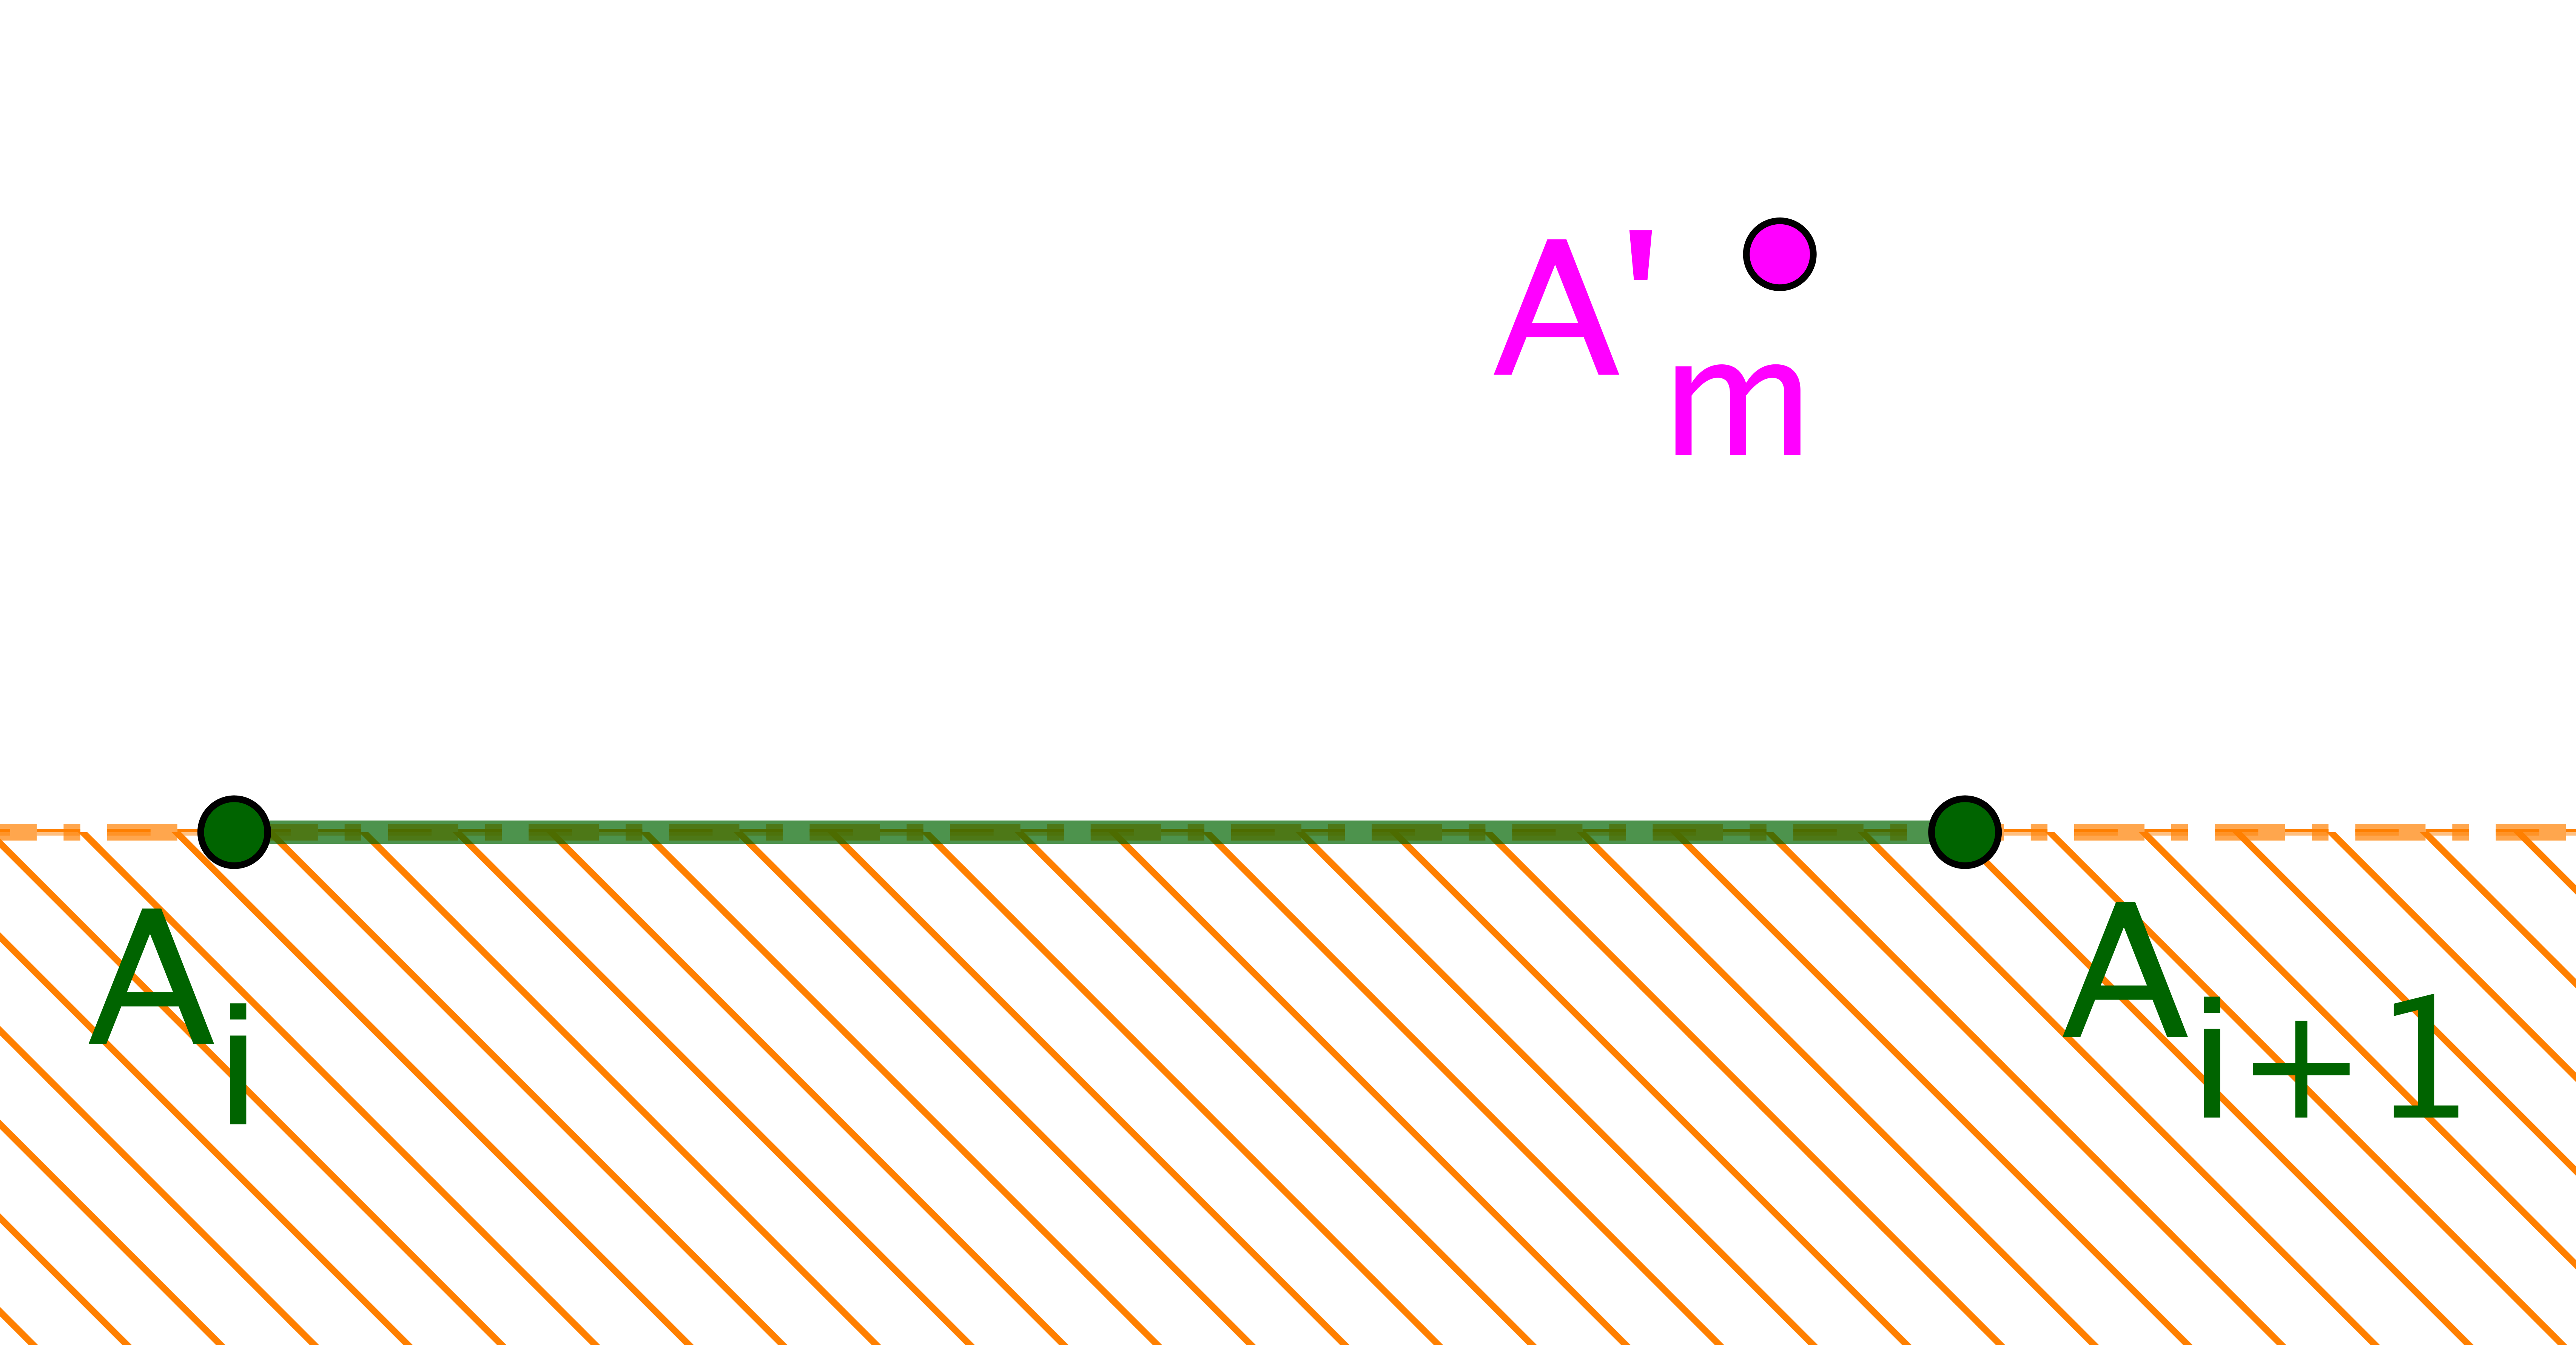
\includegraphics[scale=.2]{content/polygon/at-least-one/algo-kgone-remove-vertices.png}
        \end{center}
        
        \noindent
        Nous arrivons aux constatations suivantes.
        %
        \begin{itemize}
            \item Les points $\primeit{A}_i$, $\primeit{A}_{m-1}$ et $\primeit{A}_m$ ne sont pas alignés.

            \item Comme 
            $\forall j \in \ZintervalC{1}{n}$,
            $\det \big( \vect{\primeit{A}_{m-1} \primeit{A}_m}, \vect{\primeit{A}_{m-1} \primeit{A}_{j}} \big) \geq 0$, 
            nous avons
            $\primeit{A}_{j} \in ( \primeit{A}_i , \primeit{A}_{m-1} ]$,
            pour $j \in \ZintervalO{i}{m-1}$.%
            \footnote{
        	    Le point $\primeit{A}_{m-1}$ est le plus à droite sur notre schéma.
            }

            \item L'évaluation de l'aire algébrique via le point de calcul $\primeit{A}_{m-1}$ peut se passer des sommets $\primeit{A}_j$ pour $j \in \ZintervalO{i}{m-1}$, par raison d'alignement.

            \item Ignorer des sommets, tout en conservant l'ordre de parcours, pour former un nouveau cycle $\setproba{L}^{\,\prime}$, donne $\cyclelen{\setproba{L}^{\,\prime}} \leq \cyclelen{\setproba{L}} $.
        \end{itemize}
        
        \noindent
        Les constatations précédentes justifient l'ajout de
        $\primeit{A}_{m-1}$ à la fin de la liste $\onelist{C}$, uniquement si $\primeit{A}_{m-1}$ n'est pas dans cette liste,%
        \footnote{
        	La justification de l'algorithme, donnée un peu plus bas, montrera la possibilité d'avoir un doublon dans la liste $\onelist{C}$.
        }
        puis de poser $i = m - 2$, puisque nous augmentons $i$ de $1$ juste après.

	
		\item \label{algo-kgone-loop-back}
		Ajoutons $1$ à $i$.
		Si $i \geq n+1$, nous avons fini, sinon nous retournons à l'action \ref{algo-kgone-start}\,.
    \end{enumerate}
    

    \medskip

    
    Commençons par justifier que l'algorithme s'arrête sans entrer dans une boucle infinie.
    Tant que l'indice $m$ de l'étape \ref{algo-kgone-remove-vertices} vérifie $m \leq n$, il n'y a aucune difficulté, car $i$ augmente, et les sommets ajoutés se placent \focus{avant} l'origine $A_1$ du \ncycle\ initial $\setproba{L}$ sans empiéter sur les \focus{premiers} sommets. Supposons avoir $m \in \ZintervalO{n}{n+i}$ pour un indice $i$, avec $\primeit{A}_i$ stocké précédemment dans la liste $\onelist{C}$, et forcément $i > 1$.
    %
    \begin{itemize}
        \item Commençons par noter l'existence de $A_1$, $A_r$ et $A_s$ non alignés avec $A_r$ et $A_s$ stockés dans $\onelist{C}$.
        En effet,
        la première boucle de l'algorithme donne $A_r$, puis $A_s$ apparaît lors de la deuxième boucle.


        \item Supposons que $i = s$. 
        Pour $j \in \ZintervalC{s+1}{n}$, les points $\primeit{A}_j$ sont sur la droite $( \primeit{A}_s \primeit{A}_1)$ d'après l'algorithme, 
        puis plus généralement $\primeit{A}_j \in ( \primeit{A}_s \primeit{A}_1)$ pour $j \in \ZintervalO{s}{m}$. 
        Le schéma suivant montre sans ambigüité qu'alors
        $\primeit{A}_{m-1} = \primeit{A}_1$.%
        \footnote{
            $\primeit{A}_{m-1} \neq \primeit{A}_1$ contredirait la condition de positivité large sur les déterminants.
        }
        Dès lors, $m = n+2$, d'où l'ajout de $\primeit{A}_1$ à la fin de la liste $\onelist{C}$, puis l'arrêt de l'algorithme à l'étape suivante.
        %
        \begin{center}
        	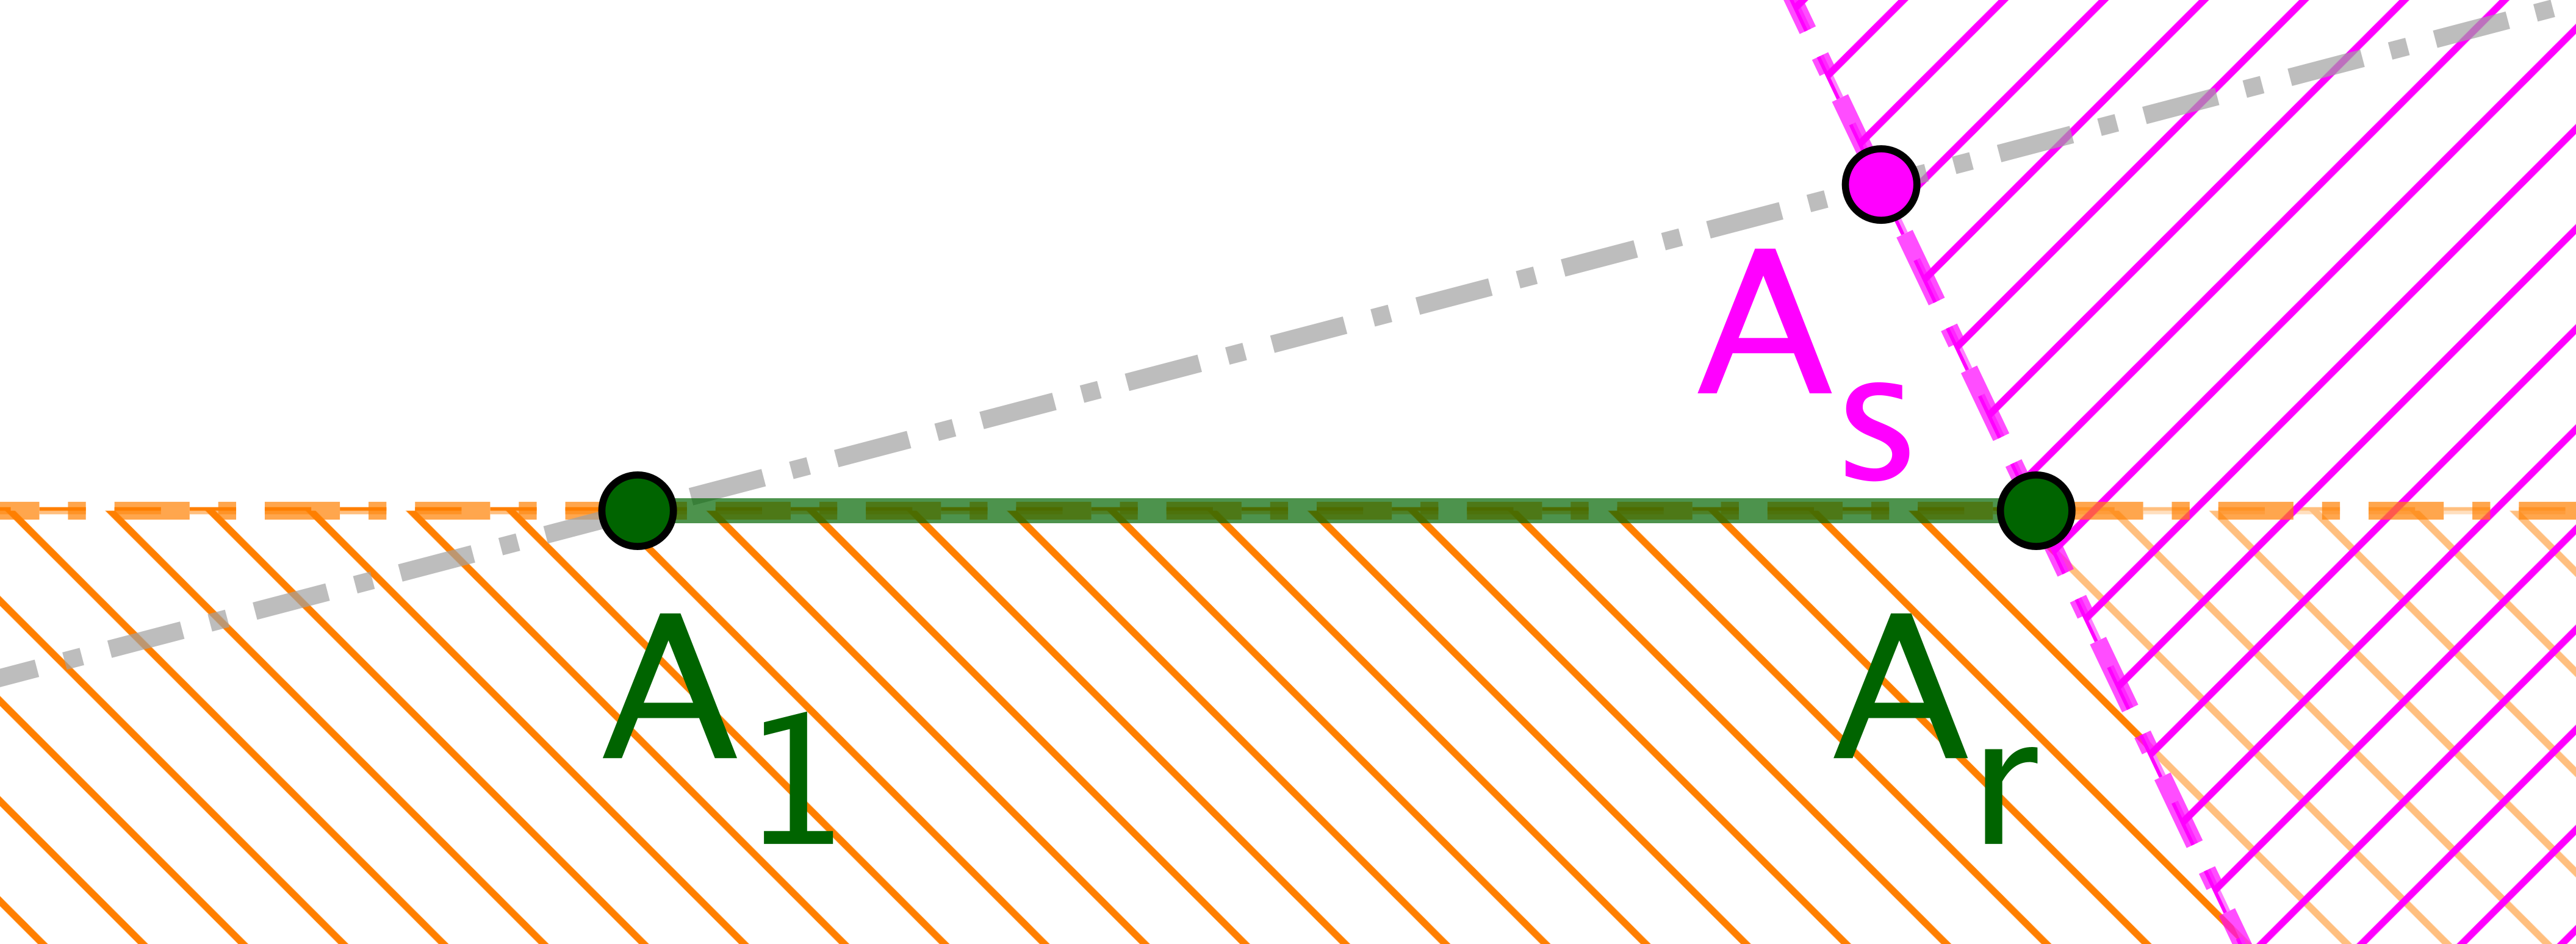
\includegraphics[scale=.2]{content/polygon/at-least-one/algo-kgone-terminate-1.png}
        \end{center}


        \item Le raisonnement précédent fonctionne aussi lorsque $\primeit{A}_i \notin (\primeit{A}_1 \primeit{A}_r)$.


        \item Il reste le cas où $\primeit{A}_i \in (\primeit{A}_1 \primeit{A}_r)$.
       	Ceci nous donne le schéma suivant, où
       	$\primeit{A}_i \in [\primeit{A}_1 \primeit{A}_r]$ est possible, a priori. 
        %
        \begin{center}
        	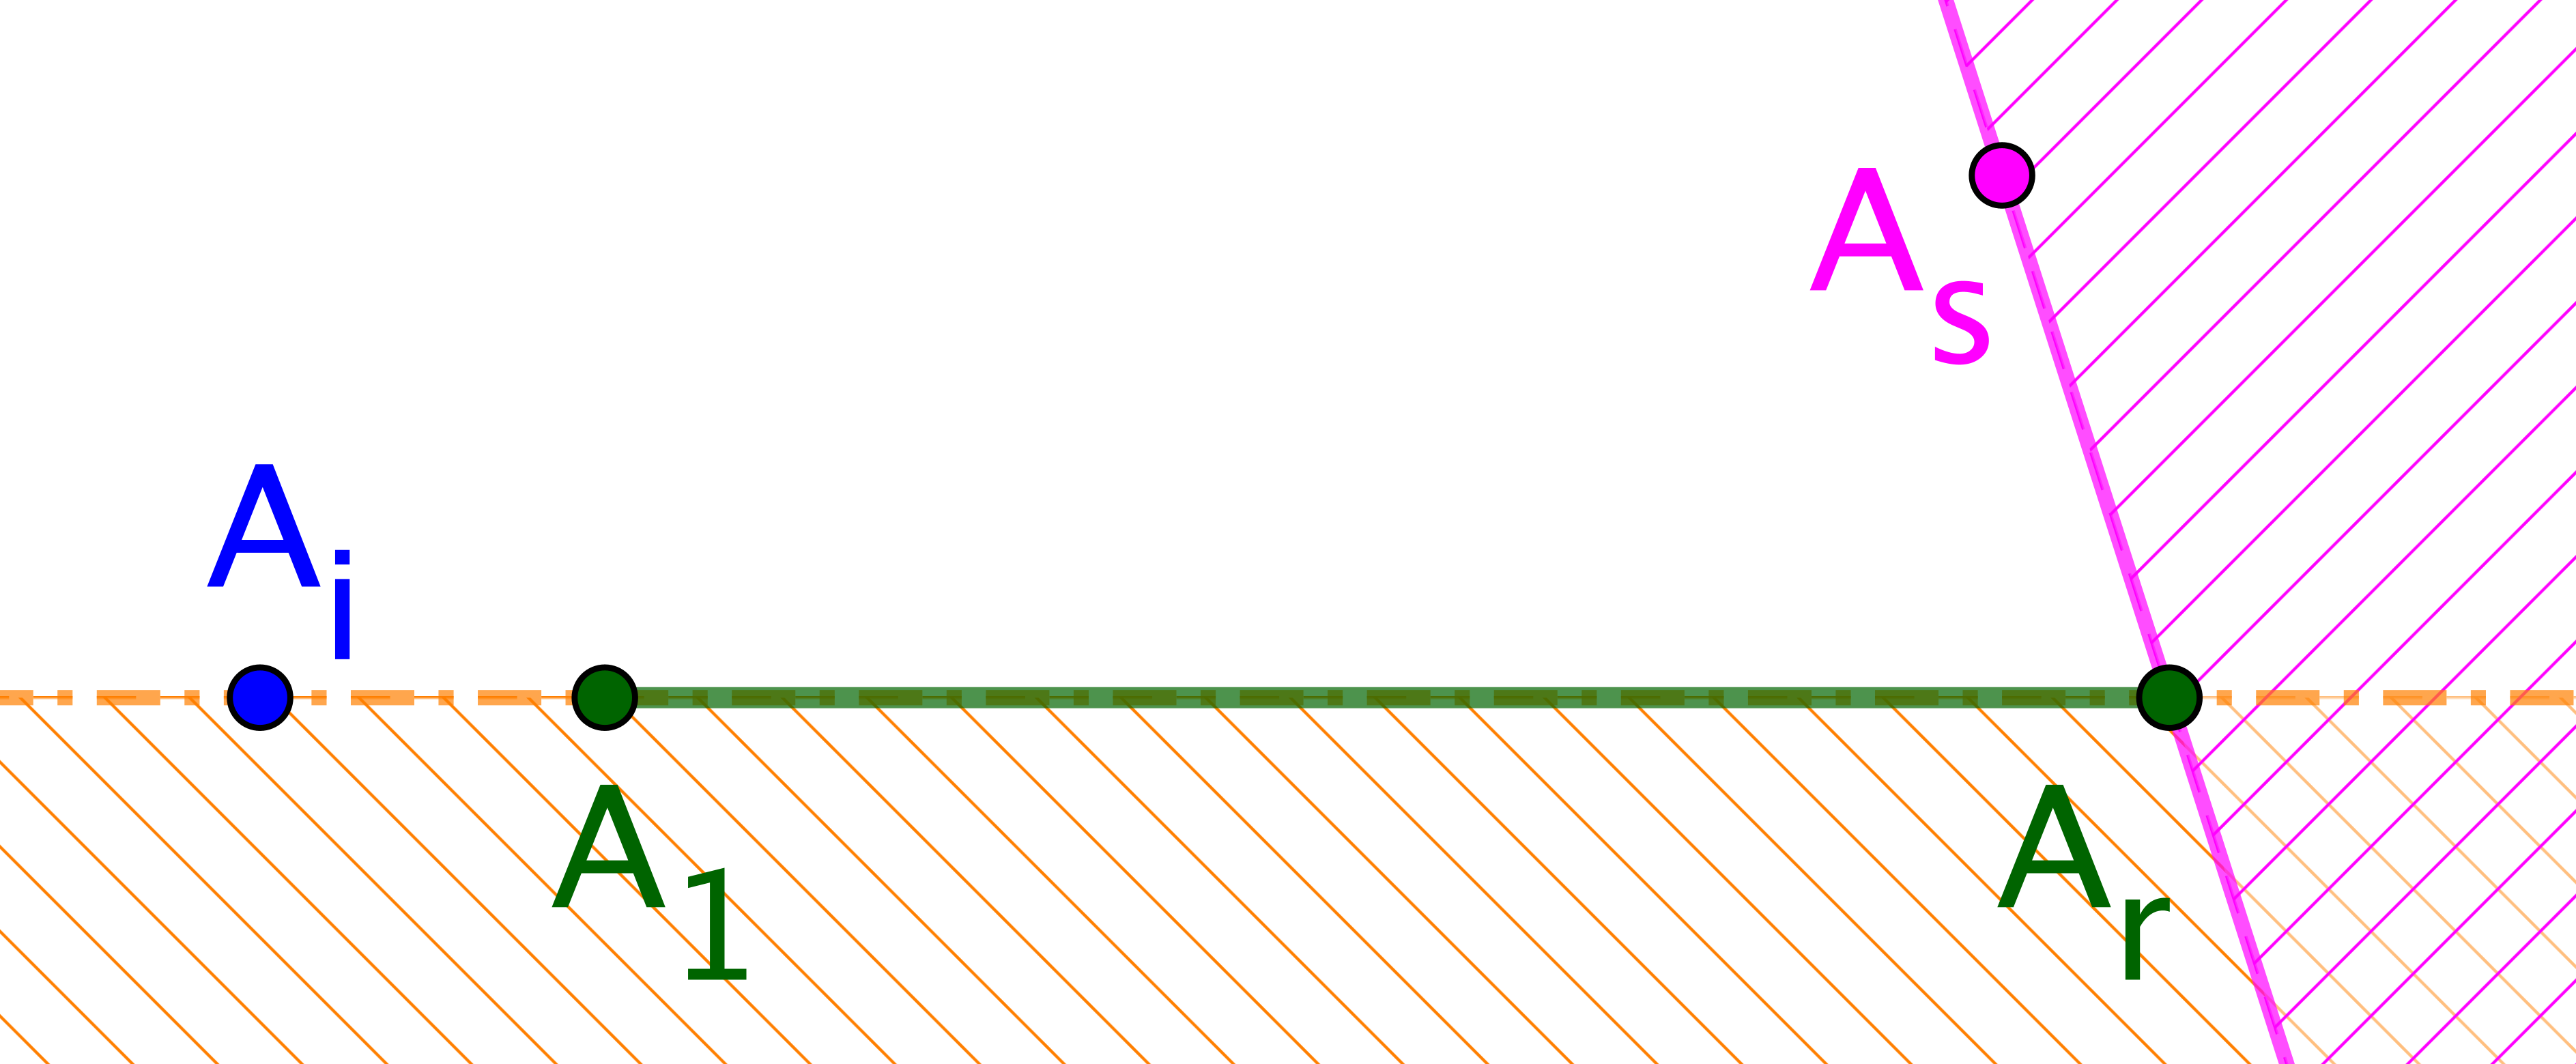
\includegraphics[scale=.2]{content/polygon/at-least-one/algo-kgone-terminate-2.png}
        \end{center}
        
        \noindent
        L'algorithme assure l'existence d'un point $\primeit{A}_p \notin ( \primeit{A}_1 , \primeit{A}_r )$ stocké dans $\onelist{C}$ et \focus{précédent} $\primeit{A}_i$,
        tel que tout point entre $\primeit{A}_p$ et $\primeit{A}_i$ soit sur $(\primeit{A}_p \primeit{A}_i)$.
        Nous arrivons au schéma plus précis ci-dessous, où
        $\primeit{A}_1 \in [ \primeit{A}_i , \primeit{A}_r ]$
        par positivité large des déterminants
        $\det \big( \vect{\primeit{A}_p \primeit{A}_{p+1}}, \vect{\primeit{A}_p \primeit{A}_k} \big)$,
        avec la possibilité d'avoir $\primeit{A}_p = \primeit{A}_s$.
        %
        \begin{center}
        	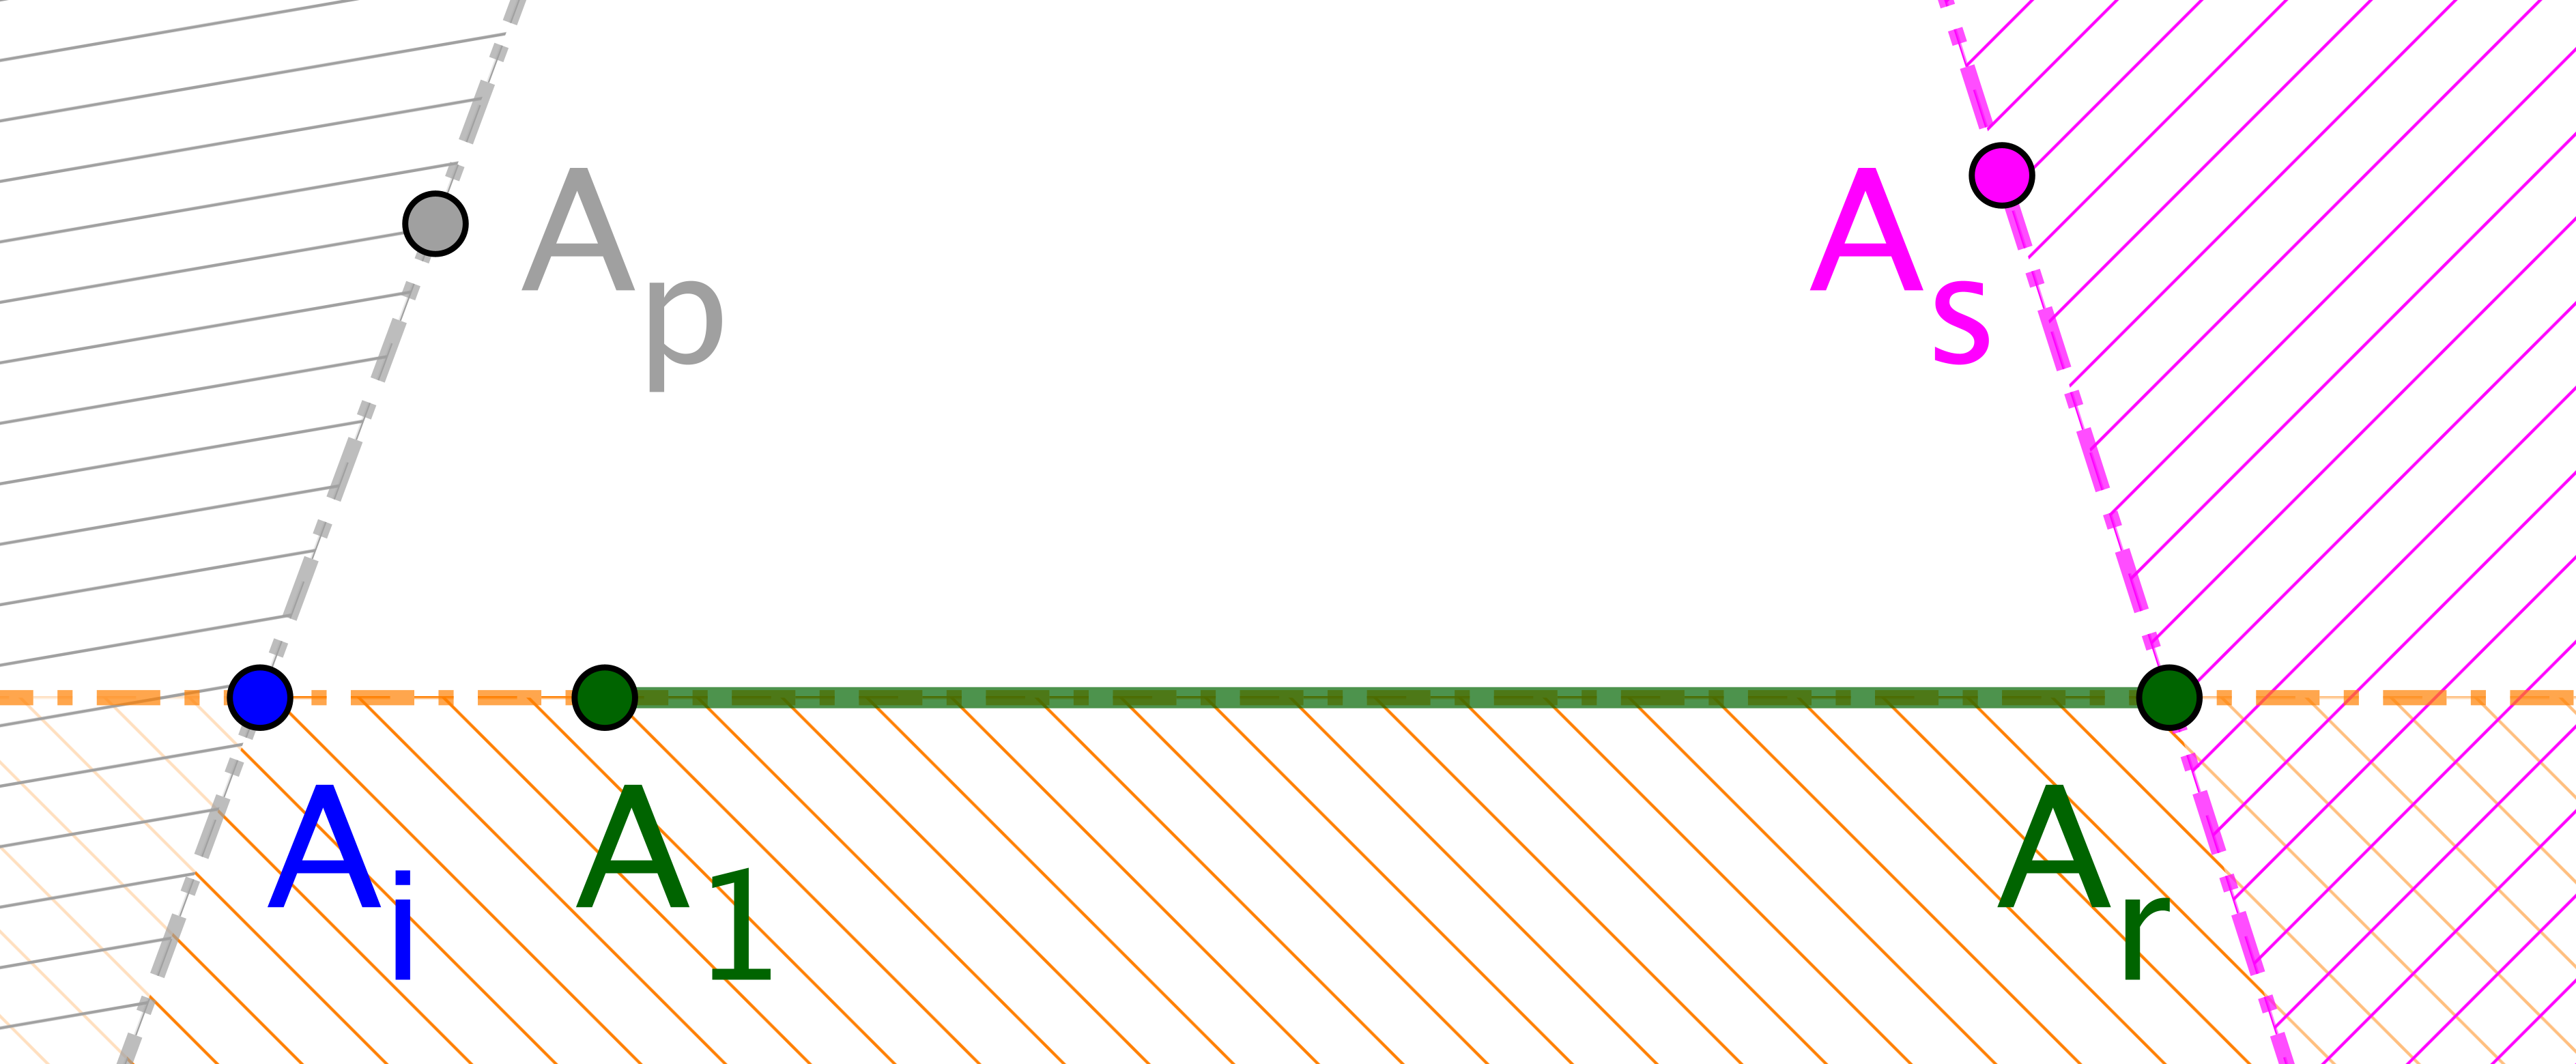
\includegraphics[scale=.4]{content/polygon/at-least-one/algo-kgone-terminate-3.png}
        \end{center}
        
        \noindent
        Ici,
        $\primeit{A}_{m-1} = \primeit{A}_r$ est déjà dans $\onelist{C}$,
        donc l'algorithme s'arrêtera après avoir juste modifié $i$ en $(n + r)$.
        Notons que les points de $\primeit{A}_{i+1}$ à $\primeit{A}_{r-1}$ sont \focus{mangés} comme attendu.
    \end{itemize}
    
    
    \medskip
    
    
    Il faut aussi justifier que la liste $\onelist{C}$, lue de gauche à droite, donnera les sommets du \kgone\ convexe $\setproba{C}$ cherché.
    %
    \begin{itemize}
        \item Par construction, deux sommets \focus{consécutifs} $\primeit{A}_r$ et $\primeit{A}_s$ de $\setproba{C}$, sont tels que tout point du cycle initial $\setproba{L}$ situé entre $\primeit{A}_r$ et $\primeit{A}_s$ se trouve sur le segment $[\primeit{A}_r \primeit{A}_s]$.
        En ignorant ces points, on fait donc diminuer, au sens large, la longueur du \ncycle, mais sans modifier la valeur de l'aire algébrique, cette dernière étant calculable depuis $\primeit{A}_r$.
        Donc
        $\cyclelen{\setproba{C}} \leq \cyclelen{\setproba{L}}$
		et
		$\sarea{\setproba{C}} = \sarea{\setproba{L}}$


        \item Par construction, trois sommets \focus{consécutifs} $\primeit{A}_q$, $\primeit{A}_r$ et $\primeit{A}_s$ de $\setproba{C}$, sont tels que $\det \big( \vect{\primeit{A}_q \primeit{A}_{r}}, \vect{\primeit{A}_q \primeit{A}_s} \big) > 0$.
        Dès lors, $\setproba{C}$ est un \kgone\ convexe d'après le fait \ref{conv-pos-det}.
    \end{itemize}

	
	Pour finir, la preuve ci-dessus de l'algorithme montre que pour $\primeit{A}_i$ et $\primeit{A}_k$ deux sommets consécutifs de $\setproba{C}$, les sommets $\big( \primeit{A}_j \big)_{ j \in \ZintervalC{i}{k} }$ sont les seuls situés sur $[\primeit{A}_i \primeit{A}_k]$.
\end{proof}


\begin{remark}
    La propriété sur les sommets donne un algorithme de construction de $\setproba{C}$, très simple, lorsque $\setproba{L}$ n'est pas totalement dégénéré.
    %
    \begin{enumerate}[label=\fbox{\small\bfseries\textsf{A\kern.25pt\arabic*}}]
        \item On pose $i = 1$, et on considère une liste vide $\onelist{C}$.

        \item \label{algo-easy-extract-conv}
              On pose $j = i + 1$,
              puis
              tant que $\primeit{A}_j = \primeit{A}_i$, on augmente $j$ de $1$.

        \item On pose $k = j + 1$,
              puis
              tant que $\primeit{A}_k \in (\primeit{A}_i \primeit{A}_j)$, on augmente $k$ de $1$.

        \item Si $\primeit{A}_k$ n'est pas dans $\onelist{C}$, on ajoute ce sommet à droite de la liste, on pose $i = k$, et on retourne à l'action \ref{algo-easy-extract-conv}. Sinon, on s'arrête.
    \end{enumerate}
\end{remark}


% ----------------------- %


%\newpage
%

Le résultat qui suit est juste là pour simplifier la démonstration du fait \ref{at-least-one-ngone-convex} à venir qui est la raison d'être de cette section.


\begin{fact} \label{at-least-one-ncycle}
    Soient $n \in \NN_{\geq3}$,
    $\ell \in \RRsp$,
    $\pvaxes{O | i | j}$ un repère orthonormé direct du plan
    et
    $\setproba{U} \subset \RR^{2n}$ l'ensemble des uplets de coordonnées $\big( x(A_1) ; y(A_1) ; \dots ; x(A_n) ; y(A_n) \big)$ où $\setproba{L} = A_1 A_2 \cdots A_n$ désigne un \ncycle\ convexe tel que $\cyclelen{\setproba{L}} = \ell$.
    %
    Dès lors, la fonction $\alpha: \setproba{U} \rightarrow \RR$, qui à un uplet de $\setproba{U}$ associe l'aire algébrique du \ncycle\ qu'il représente, est une fonction admettant au moins un maximum, qui est positif strict.
    %
    De plus, un \ncycle\ maximisant $\alpha$ est forcément un \ngone\ convexe.
\end{fact}


\begin{proof}
     $\setproba{U}$ est fermé dans $\RR^{2n}$, car les conditions le définissant le sont, et il est borné, car inclus dans la boule fermée de centre $\pt{O}$ et de rayon $\ell$,
     donc $\setproba{U}$ est un compact de $\RR^{2n}$.
     De plus, $\alpha$ est continue d'après le fait \ref{sarea-cont}.
     Donc, par continuité et compacité, $\alpha$ admet un maximum sur $\setproba{U}$, celui-ci étant positif strict pour les raisons suivantes où $\setproba{R}$ désigne un \nreg\ convexe.
    %
    \begin{itemize}
		\item Via une translation, nous pouvons supposer $\setproba{R}$ d'origine $\pt{O}$.

        \item $\area{\setproba{R}} = \abs{\sarea{\setproba{R}}}$
		selon le fait \ref{sarea-ngone},
		et
		$\sarea{\setproba{R}^{\mathrm{op}}} = - \sarea{\setproba{R}}$ d'après le fait \ref{nline-rota-opp}.
		
		\item $\setproba{R} \in \setproba{U}$, ou $\setproba{R}^{\mathrm{op}} \in \setproba{U}$ par convexité.
		
		\item Si $\setproba{R} \in \setproba{U}$, alors 
		$\setproba{R}$ est orienté positivement, 
		d'où $\sarea{\setproba{R}} \geq 0$, 
		et par conséquent $\sarea{\setproba{R}} = \area{\setproba{R}}$ 
		(ceci se démontre aisément en utilisant le centre de gravité de $\setproba{R}$ comme point de calcul). 
		Nous avons une propriété similaire si $\setproba{R}^{\mathrm{op}} \in \setproba{U}$.

        \item Enfin, il est connu, et très facile de démontrer, que tout \nreg\ convexe $\setproba{R}$ vérifie
        $\cyclelen{\setproba{R}} = 2 n \sin (\frac{\pi}{n}) \rho$
		et
		$\area{\setproba{R}} = n \sin (\frac{\pi}{n})  \cos (\frac{\pi}{n}) \rho^2$
		où $\rho$ est le rayon du cercle circonscrit à $\setproba{R}$.
		Il existe donc un \nreg\ convexe $\setproba{R}$ de longueur $\ell$, et forcément d'aire non nulle.
    \end{itemize}

    
    Pour finir, justifions qu'un \ncycle\ $\setproba{M} \in \setproba{U}$ maximisant $\alpha$ est forcément un \ngone\ convexe. 
    Comme $\sarea{\setproba{M}} > 0$, $\setproba{M}$ n'est pas totalement dégénéré,
    donc nous pouvons considérer le \kgone\ convexe $\setproba{C}$ donné par le fait \ref{conv-from-non-neg-det}.
    Via des arguments similaires à ceux utilisés pour $\setproba{R}$, 
    nous avons $\area{\setproba{C}} = \sarea{\setproba{C}} = \sarea{\setproba{M}}$.
    De plus,
    $0 < \cyclelen{\setproba{C}} \leq \cyclelen{\setproba{M}}$.
    %
    \begin{itemize}
		\item Supposons d'abord $k = n$.
		Si $\cyclelen{\setproba{C}} = \cyclelen{\setproba{M}}$, nous n'avons rien à faire.
		En fait, $\cyclelen{\setproba{C}} < \cyclelen{\setproba{M}}$ est impossible, 
		car une homothétie de rapport $r > 1$, où l'on a posé $r = \frac{ \cyclelen{\setproba{M}} }{ \cyclelen{\setproba{C}} }$, donnerait un \ngone\ convexe $\primeit{\setproba{C}}$ vérifiant
		$\cyclelen{\primeit{\setproba{C}}} = \cyclelen{\setproba{M}}$
		et
		$\sarea{\primeit{\setproba{C}}} > \sarea{\setproba{M}}$, ceci contredisant la maximalité de $\setproba{M}$.


		\item Pour la suite, nous supposons $k < n$, et considérons $A$, $B$ et $C$, trois sommets consécutifs, forcément distincts, du \kgone\ $\setproba{C}$. 


		\item Par convexité de $\setproba{C}$, nous avons l'une des deux configurations génériques suivantes où les demi-droites en pointillés, portées par les côtés contigus à $[AB]$, \focus{dessinent} avec $[AB]$ une région hachurée $\setproba{H}$ qui est ouverte et à l'extérieur de $\setproba{C}$. 
		Sans perte de généralité, nous allons travailler avec la 1\iere\ configuration (qui laisse moins de liberté géométrique).
		%
		\begin{multicols}{2}
			\centering

			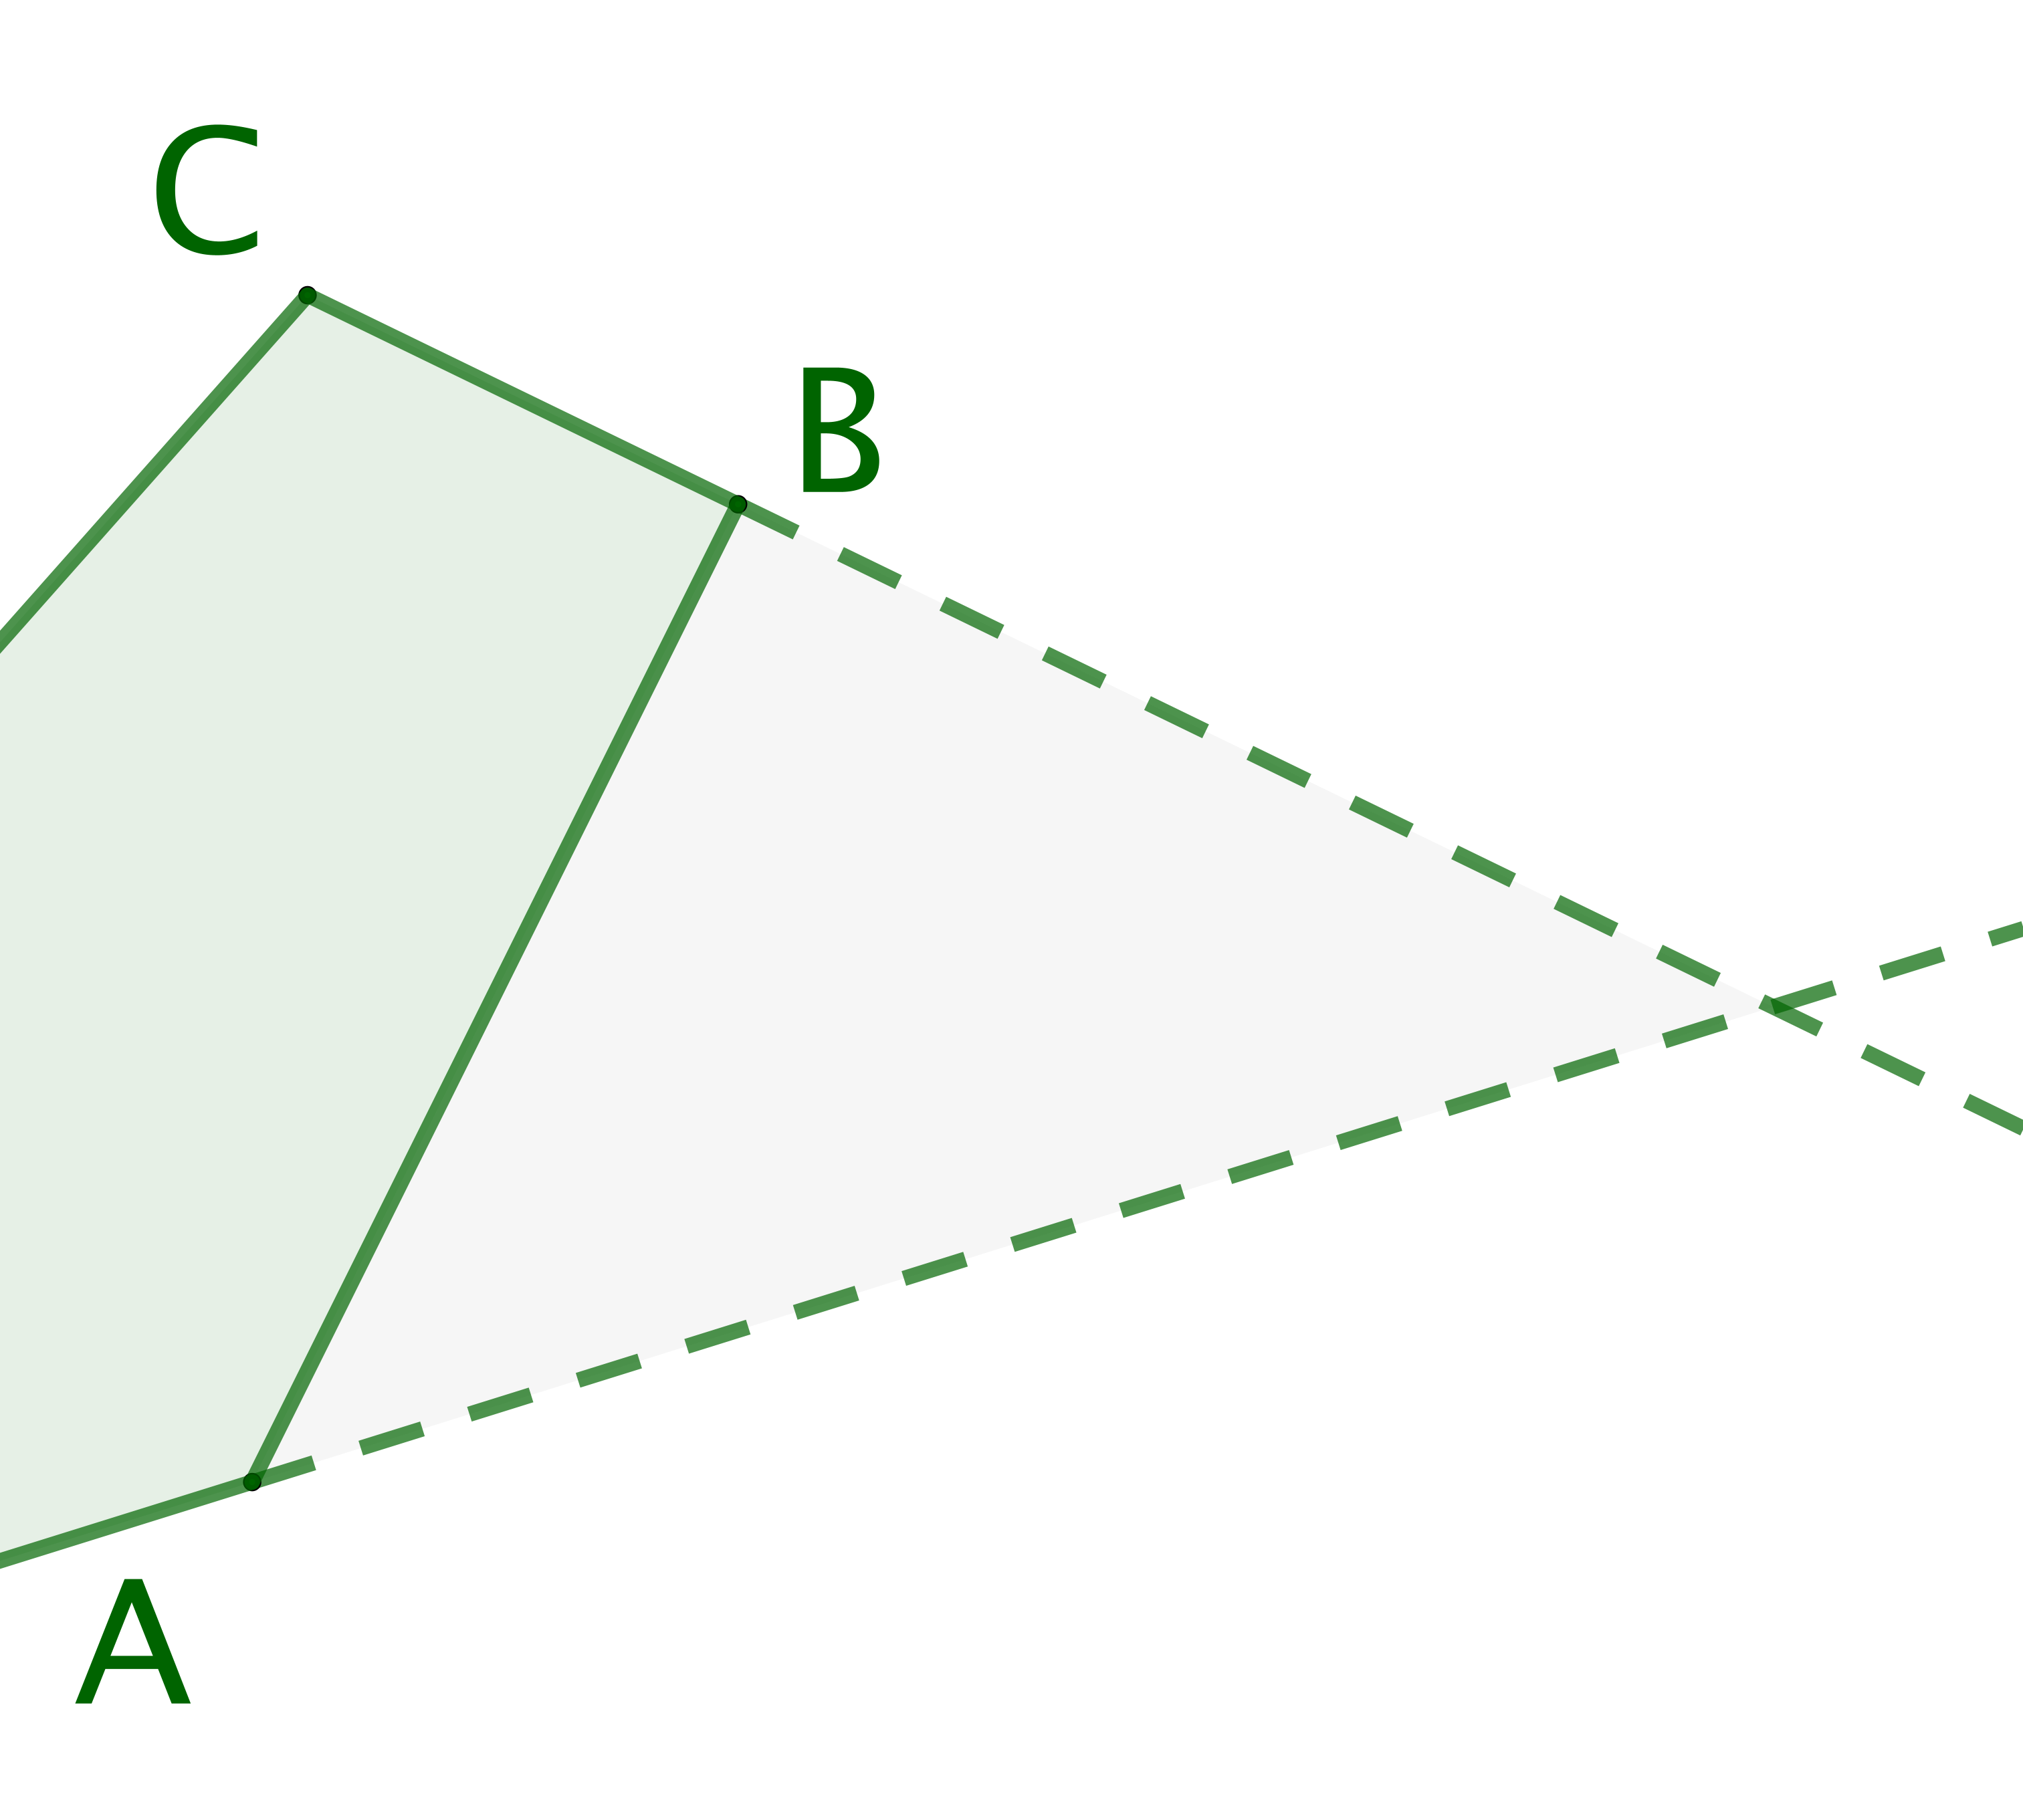
\includegraphics[scale=.35]{content/polygon/at-least-one/add-vertex-1.png}

			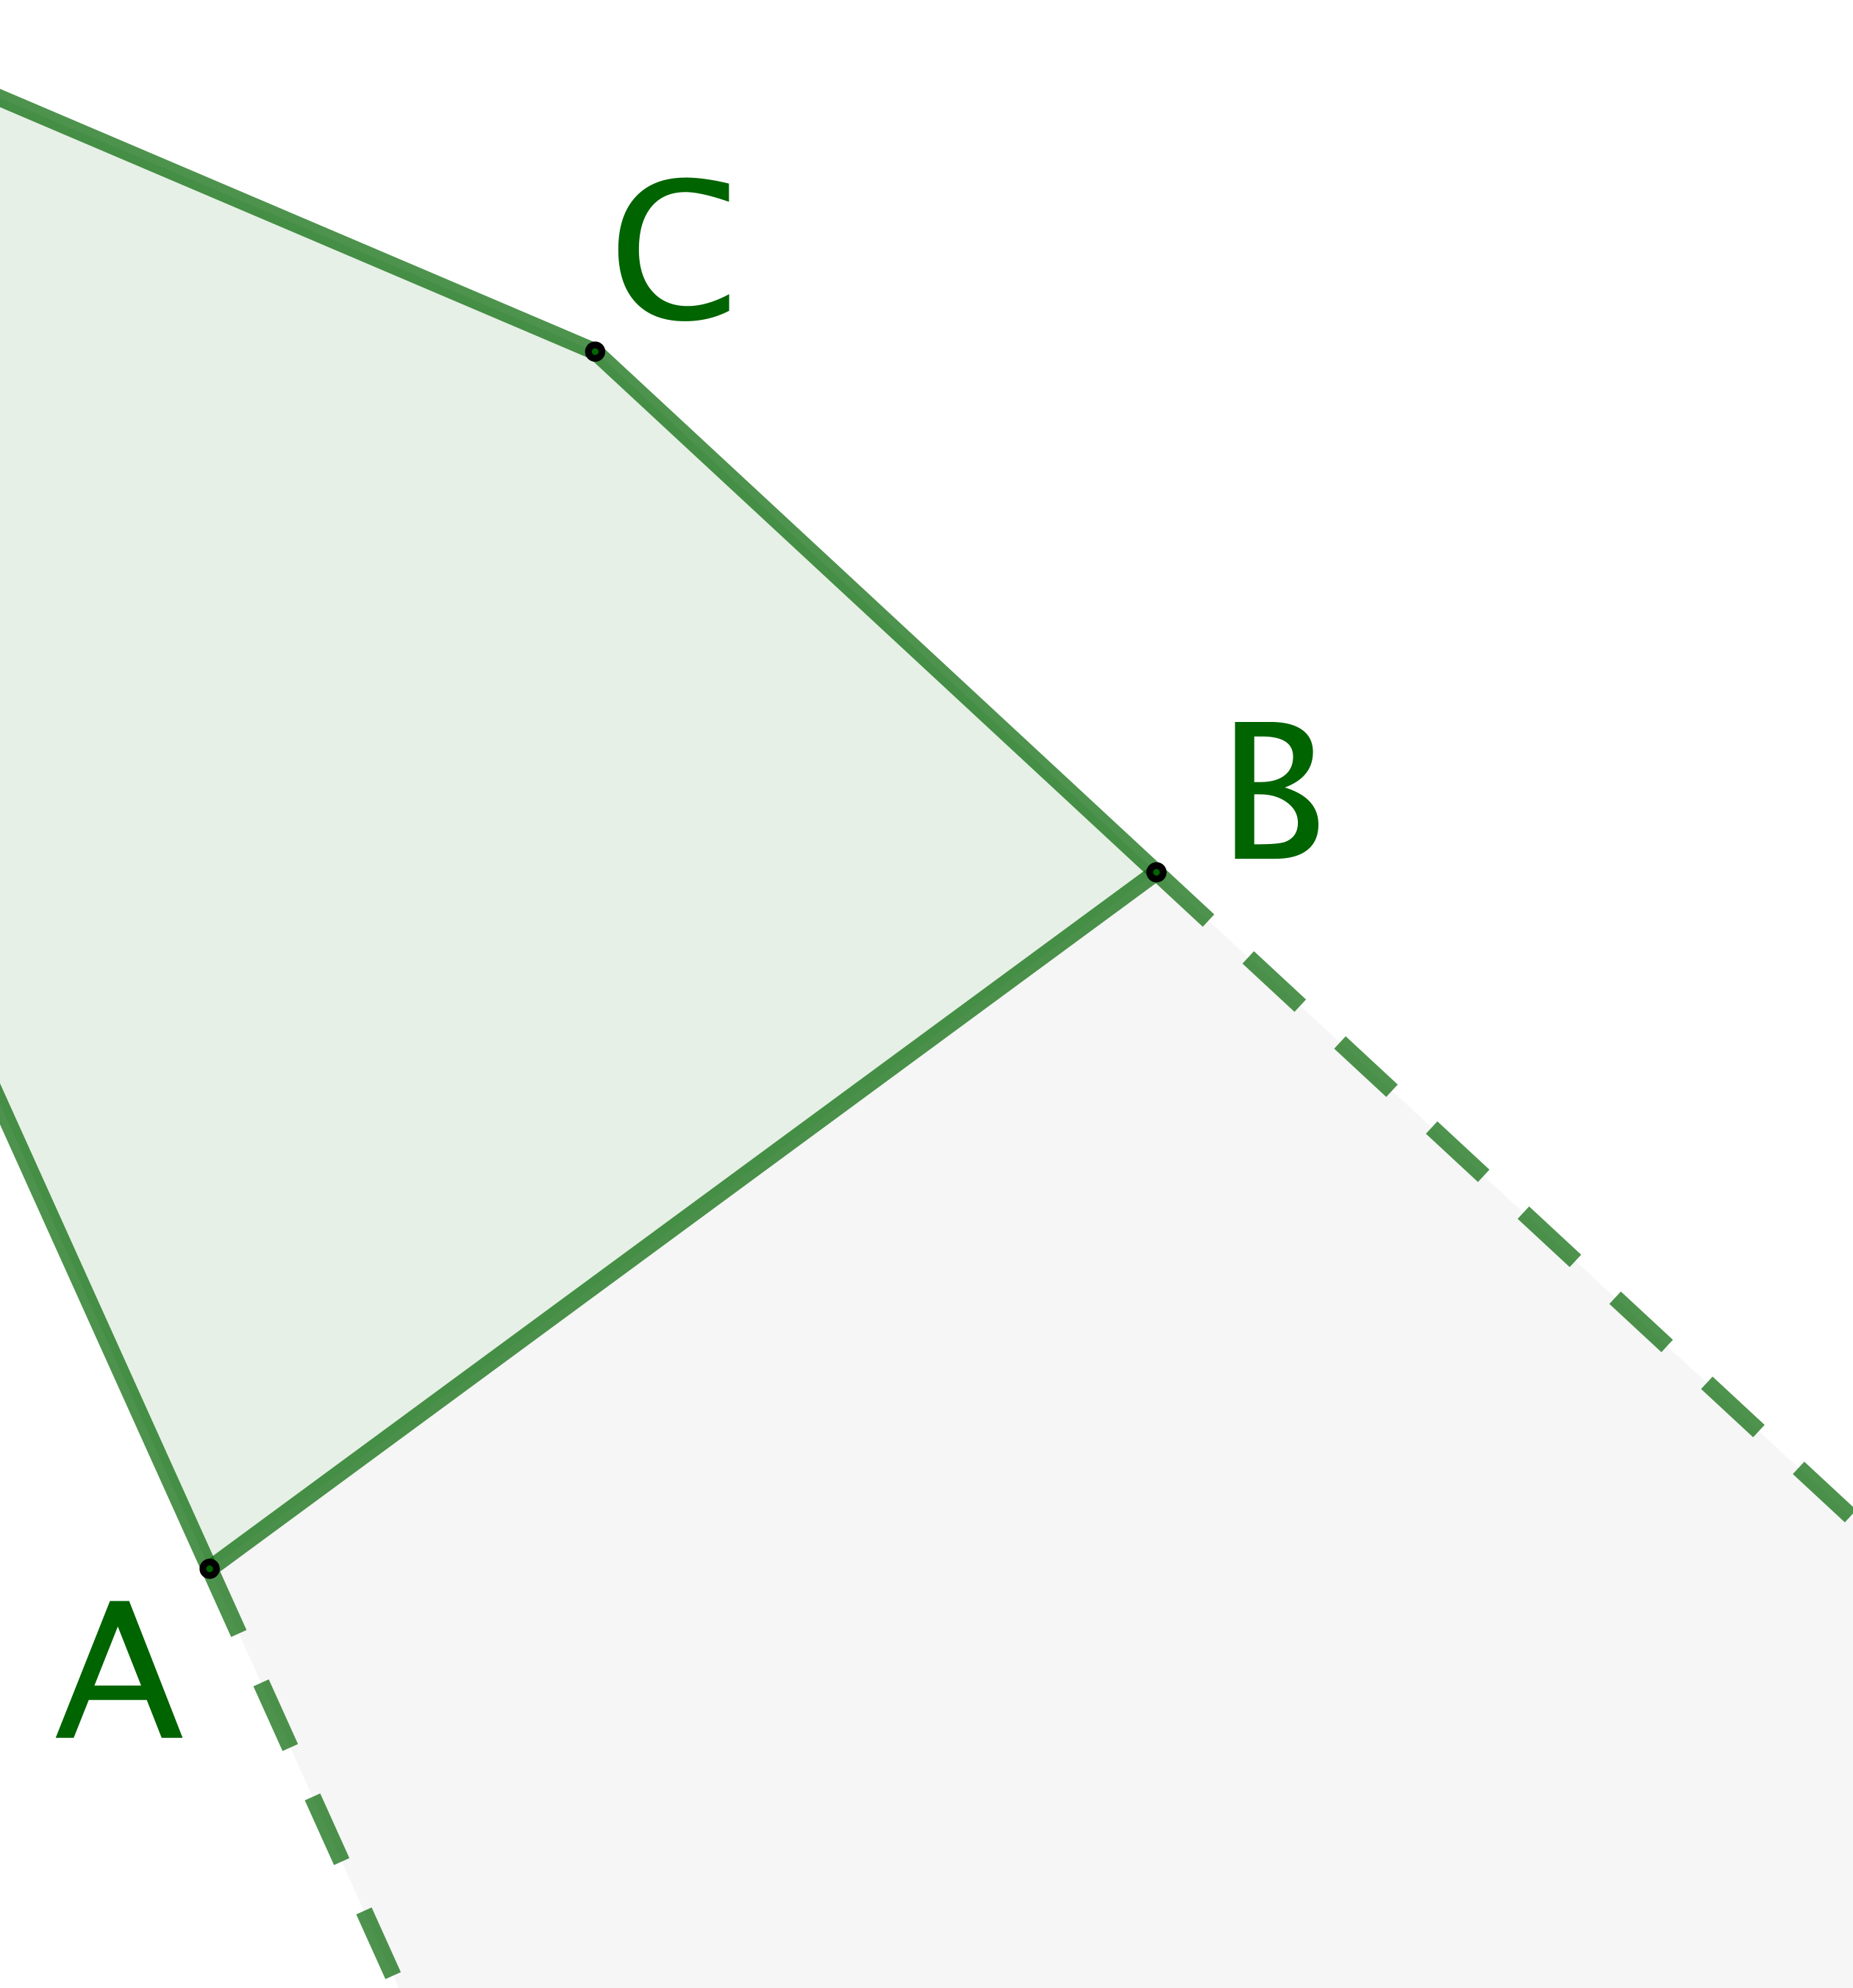
\includegraphics[scale=.35]{content/polygon/at-least-one/add-vertex-2.png}
		\end{multicols}


		\item Considérons alors $M \in {]BC[}$ quelconque pour le moment.
		Définissons ensuite le point $\primeit{B}$ par les contraintes $(B \primeit{B}) \parallel (AM)$
		et
		$\primeit{B} \in d$, où $d$ est la droite portant le côté contenant $A$ et contigu à $[AB]$.
		Par convexité, $]B \primeit{B}[$ est inclus dans la zone $\setproba{H}$.
		La figure suivante représente cette situation.
		%
		\begin{center}
			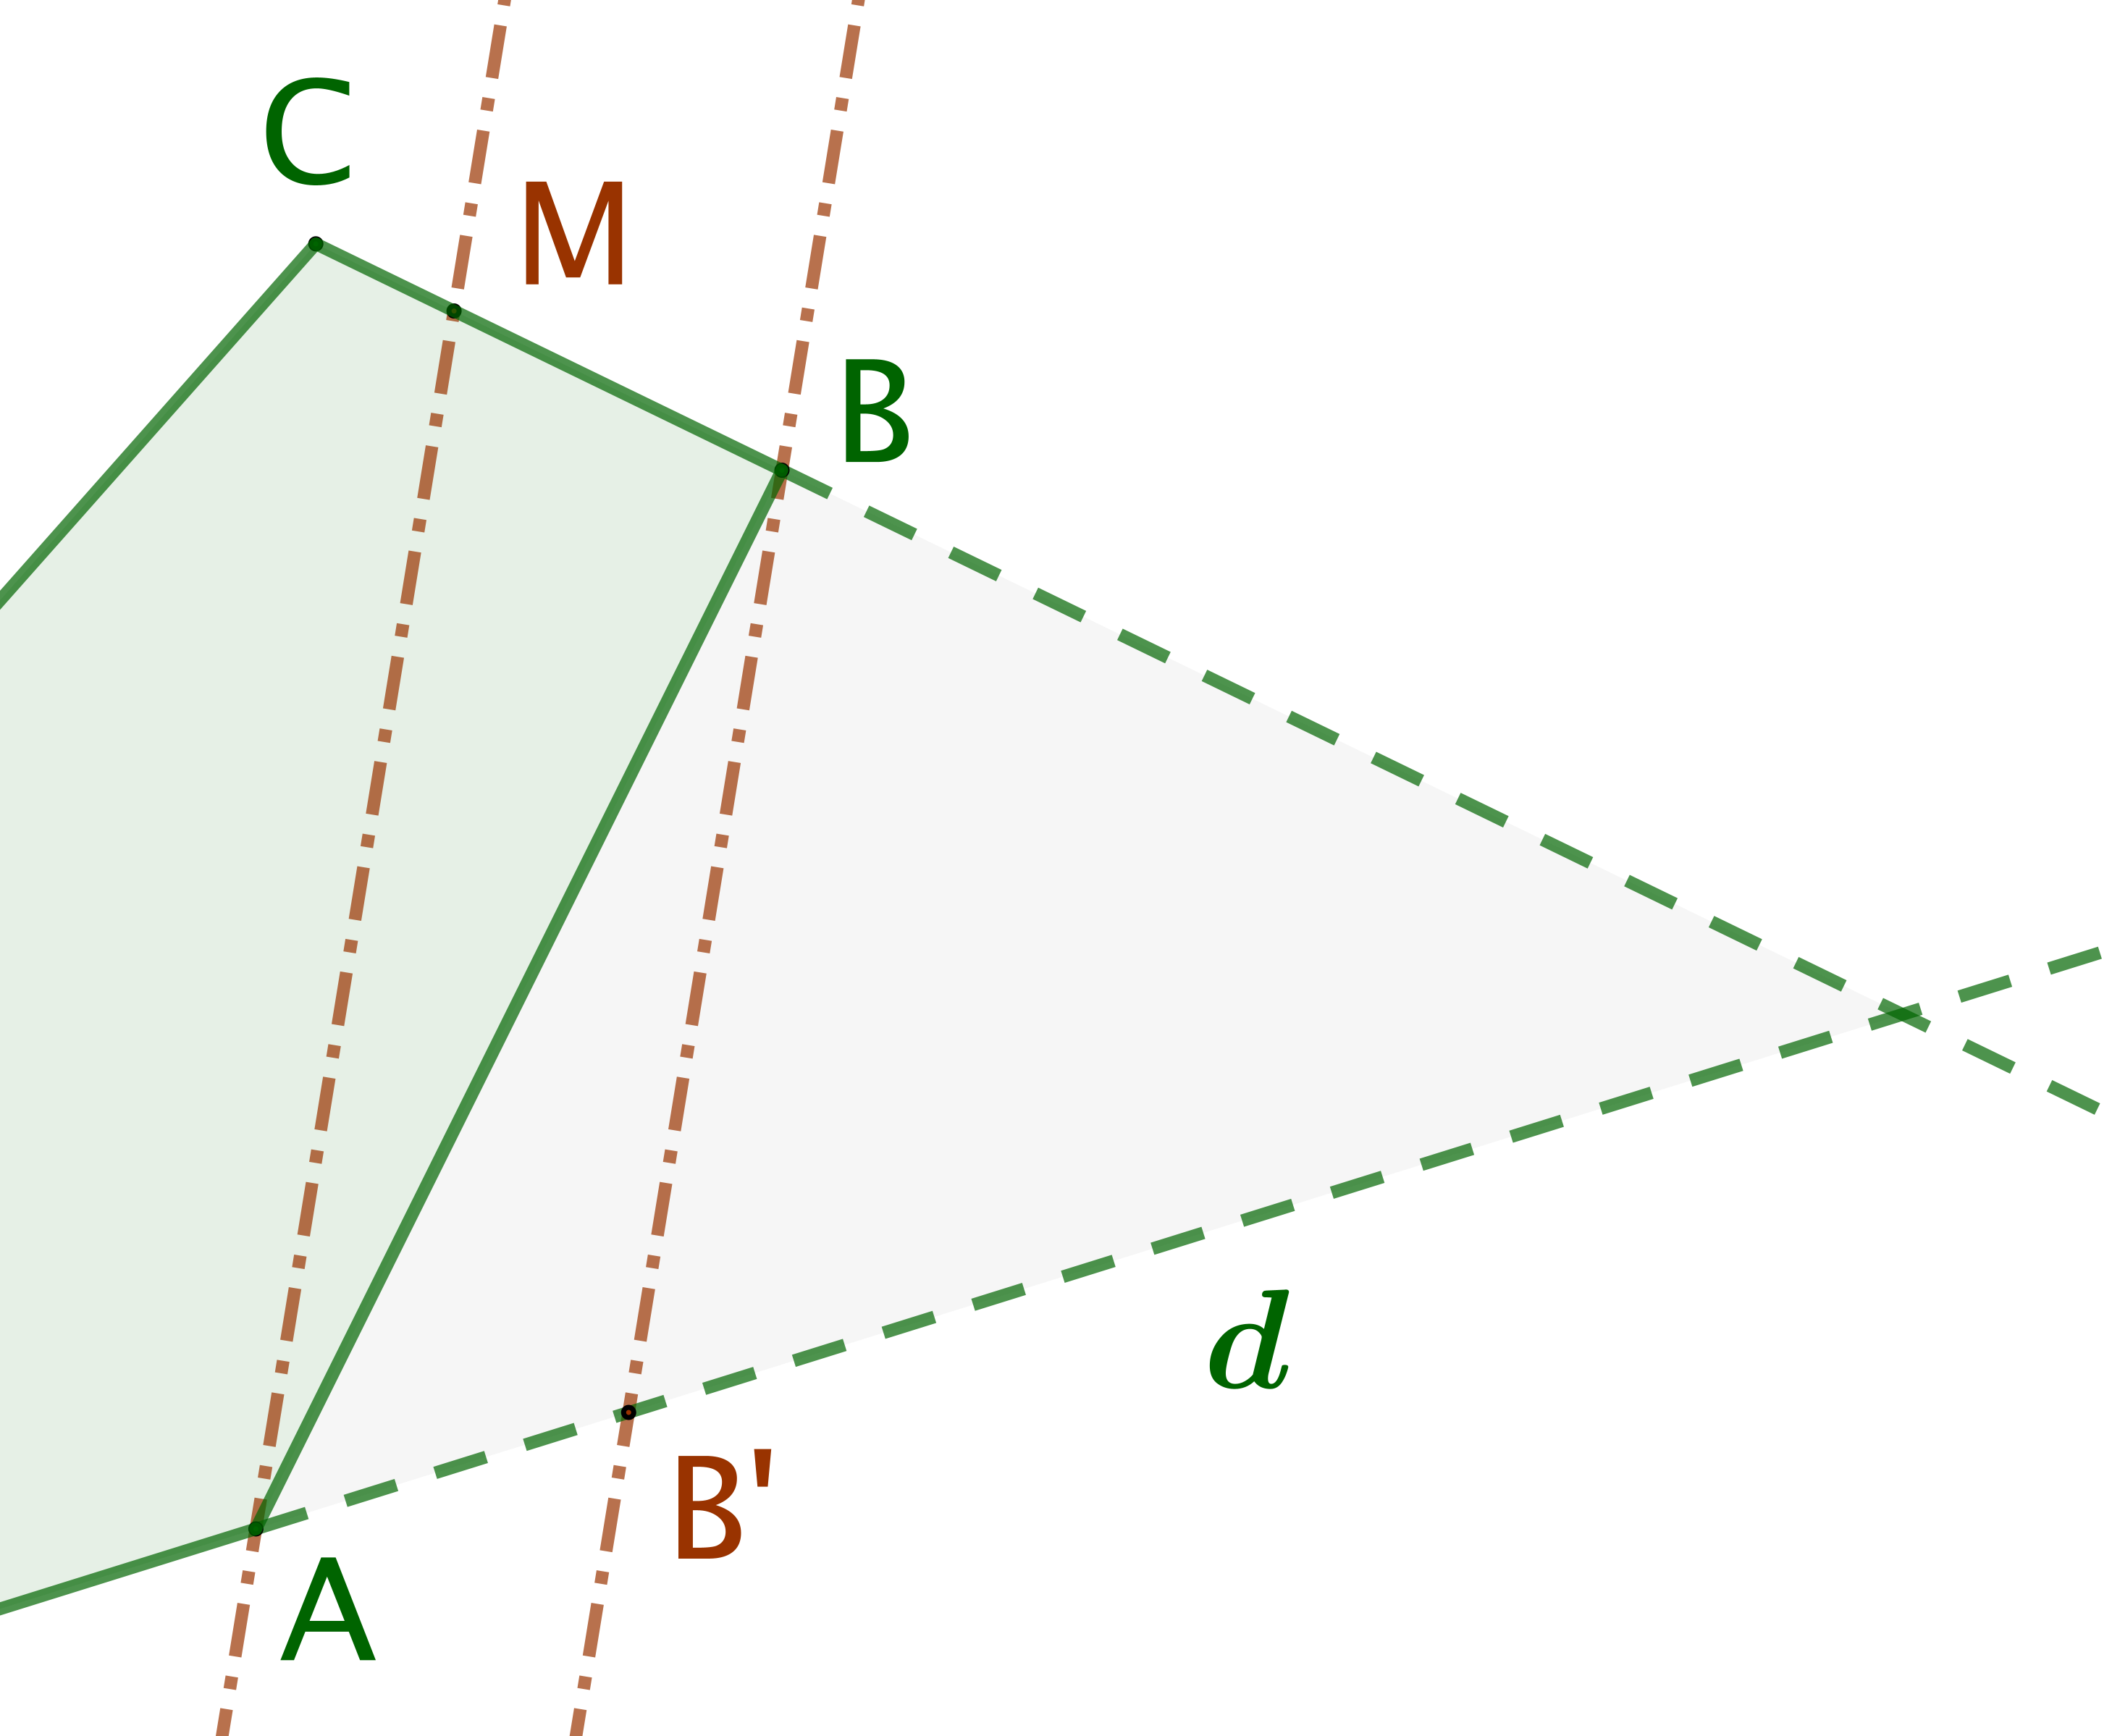
\includegraphics[scale=.4]{content/polygon/at-least-one/add-vertex-1-1.png}
		\end{center}
		


		\item Avec la preuve du fait \ref{tri-one-side-fixed} en tête, nous allons imposer d'avoir $BM < AB$, ce qui est toujours possible.
		Dès lors,
		nommons $m$ la médiatrice du segment $[AM]$,
		puis prenons $\dbleprimeit{B} \in {]B \primeit{B}[}$ plus proche de $m$ que $B$,%
		\footnote{
		    Le choix d'avoir $BM < AB$ donne l'existence de $\dbleprimeit{B}$.
		    Par contre, rien n'interdit à $m$ et $]B \primeit{B}[$ de ne jamais se croiser.
		}
		les conditions suivantes sont validées (voir la figure \focus{zoomée} juste après).
		%
		\begin{enumerate}
			\item $A \dbleprimeit{B} + M \dbleprimeit{B} < AB + MB$ par diminution du périmètre.

			\item $\area{AM \dbleprimeit{B}} = \area{AMB}$ par conservation de l'aire.

			\item En \focus{remplaçant} dans $\setproba{C}$ le sommet $B$ par $\dbleprimeit{B}$ et $M$,
		nous avons un \xgone{(k+1)} convexe $\primeit{\setproba{C}}$.
		\end{enumerate}
		%
		\begin{center}
			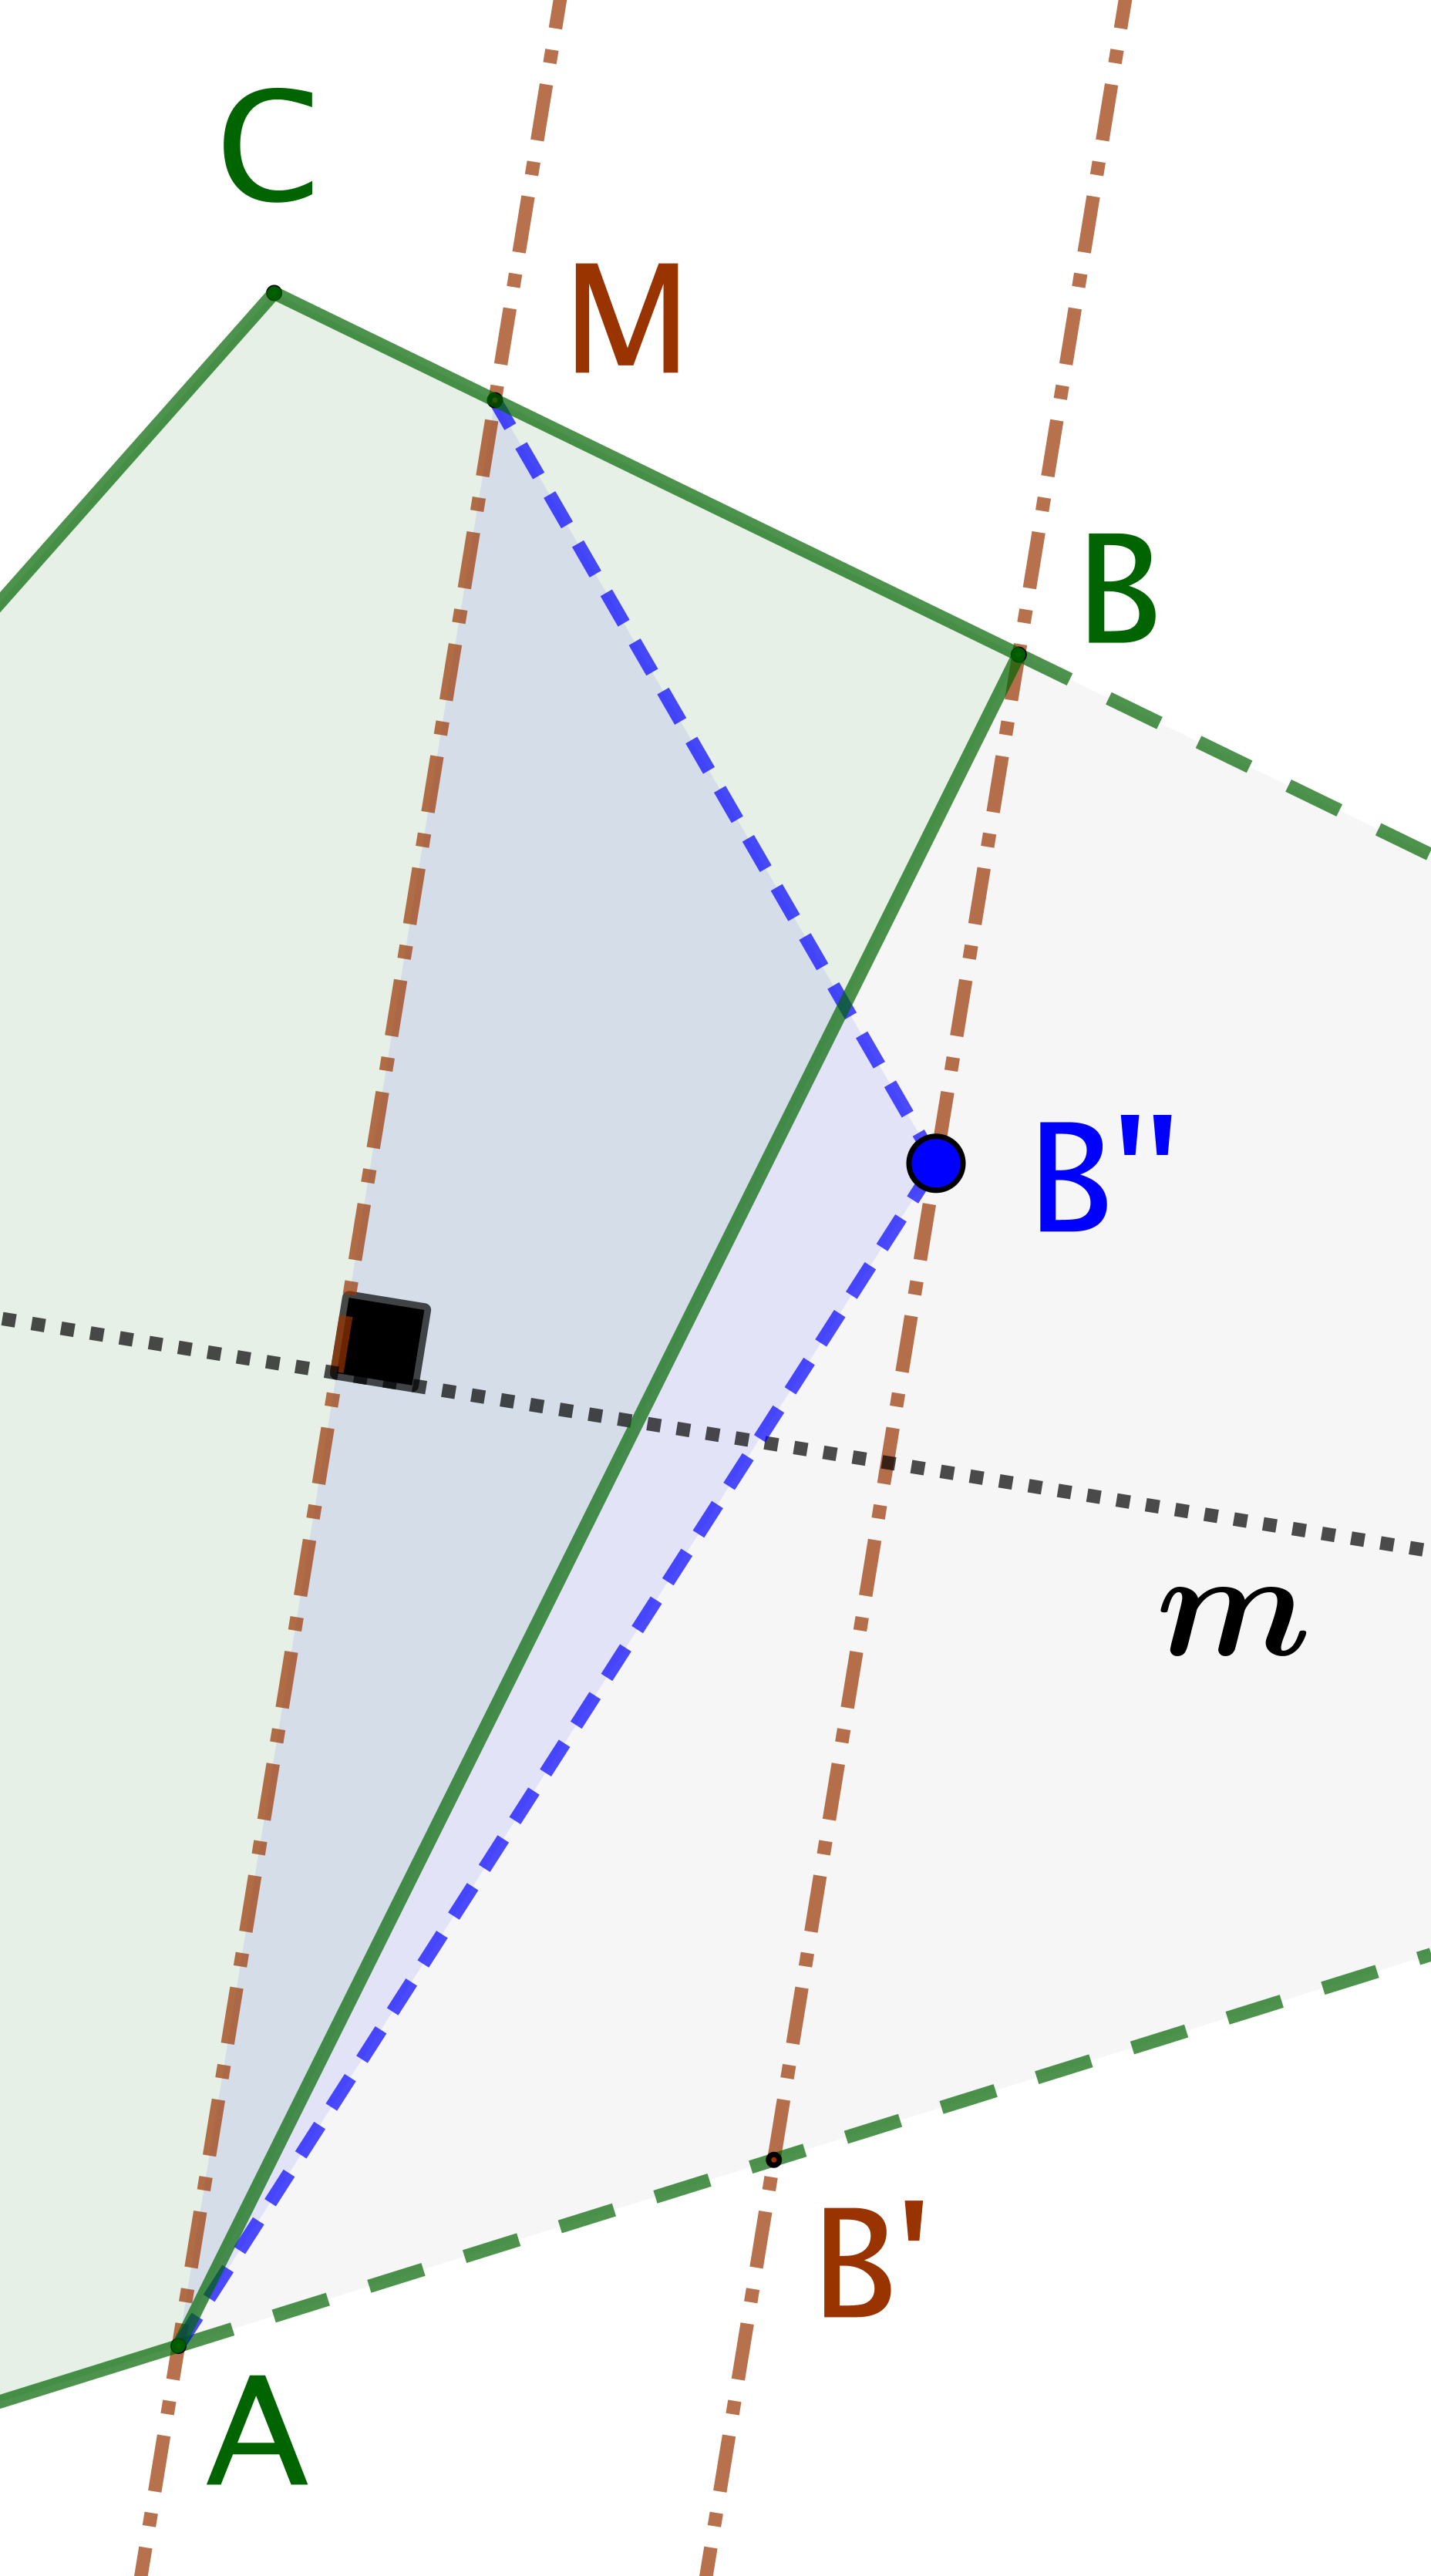
\includegraphics[scale=.4]{content/polygon/at-least-one/add-vertex-1-2.png}
		\end{center}


		\item $\primeit{\setproba{C}}$ vérifie
		$\cyclelen{\primeit{\setproba{C}}} < \cyclelen{\setproba{C}} \leq \cyclelen{\setproba{M}}$
		et
		$\area{\primeit{\setproba{C}}} = \area{\setproba{C}} = \sarea{\setproba{M}}$.


		\item En répétant $(n - k - 1)$ fois de plus les étapes précédentes, avec $\primeit{\setproba{C}}$ à la place de $\setproba{C}$ à chaque fois,
		nous obtenons un \ngone\ convexe $\dbleprimeit{\setproba{C}}$
		tel que
		$\cyclelen{\dbleprimeit{\setproba{C}}} < \cyclelen{\setproba{M}}$
		et
		$\sarea{\dbleprimeit{\setproba{C}}} = \sarea{\setproba{M}}$.
		Or, nous savons ceci impossible, donc $k < n$ ne se peut pas.
    \end{itemize}

	\null\vspace{-6ex}
\end{proof}


% ----------------------- %


Nous arrivons au résultat fondamental sur les \ngones\ convexes.


\begin{fact} \label{at-least-one-ngone-convex}
    Soit $n \in \NN_{\geq3}$ un naturel fixé.
    Parmi les \ngones\ convexes de longueur fixée, non nulle, il en existe au moins un d'aire maximale.
\end{fact}


\begin{proof}
    Soit un \ngone\ convexe $\setproba{P}$ ayant la longueur fixée. 
    %
    Pour les mêmes raisons que le \nreg\ $\setproba{R}$ utilisé dans la preuve du fait \ref{at-least-one-ncycle},
	nous pouvons supposer avoir
	soit $\setproba{P} \in \setproba{U}$ et $\sarea{\setproba{P}} = \area{\setproba{P}}$,
	soit $\cycleop{P} \in \setproba{U}$ et $\sarea{\cycleop{P}} = \area{\cycleop{P}}$.
	Comme, de plus, $\area{\cycleop{P}} = \area{\setproba{P}}$,
	nous pouvons supposer que $\setproba{P} \in \setproba{U}$,
	quitte à échanger $\setproba{P}$ et $\cycleop{P}$.
    Dès lors, il suffit de faire appel au fait \ref{at-least-one-ncycle} pour conclure.    
\end{proof}
